% !TEX TS-program = pdflatex
% !TEX encoding = UTF-8 Unicode

\documentclass[11pt]{article} % use larger type; default would be 10pt

\usepackage[utf8]{inputenc} % set input encoding (not needed with XeLaTeX)

%%% Examples of Article customizations
% These packages are optional, depending whether you want the features they provide.
% See the LaTeX Companion or other references for full information.

%%% PAGE DIMENSIONS
\usepackage{geometry} % to change the page dimensions
\geometry{a4paper} % or letterpaper (US) or a5paper or....
% \geometry{margin=2in} % for example, change the margins to 2 inches all round
% \geometry{landscape} % set up the page for landscape
%   read geometry.pdf for detailed page layout information

\usepackage{graphicx} % support the \includegraphics command and options

% \usepackage[parfill]{parskip} % Activate to begin paragraphs with an empty line rather than an indent

%%% PACKAGES
\usepackage{hyperref}
\hypersetup{
    colorlinks=true,
    linkcolor=blue,
    filecolor=magenta,      
    urlcolor=cyan,
}
\usepackage{booktabs} % for much better looking tables
\usepackage{array} % for better arrays (eg matrices) in maths
\usepackage{paralist} % very flexible & customisable lists (eg. enumerate/itemize, etc.)
\usepackage{verbatim} % adds environment for commenting out blocks of text & for better verbatim
\usepackage{subfig} % make it possible to include more than one captioned figure/table in a single float
% These packages are all incorporated in the memoir class to one degree or another...

%%% HEADERS & FOOTERS
\usepackage{fancyhdr} % This should be set AFTER setting up the page geometry
\pagestyle{fancy} % options: empty , plain , fancy
\renewcommand{\headrulewidth}{0pt} % customise the layout...
\lhead{}\chead{}\rhead{}
\lfoot{}\cfoot{\thepage}\rfoot{}

%%% SECTION TITLE APPEARANCE
\usepackage{sectsty}
\allsectionsfont{\sffamily\mdseries\upshape} % (See the fntguide.pdf for font help)
% (This matches ConTeXt defaults)

%%% ToC (table of contents) APPEARANCE
\usepackage[nottoc,notlof,notlot]{tocbibind} % Put the bibliography in the ToC
\usepackage[titles,subfigure]{tocloft} % Alter the style of the Table of Contents
\graphicspath{ {./data/photos/} }
\renewcommand{\cftsecfont}{\rmfamily\mdseries\upshape}
\renewcommand{\cftsecpagefont}{\rmfamily\mdseries\upshape} % No bold!

\urlstyle{same}
%%% END Article customizations

%%% The "real" document content comes below...

\title{Aero Multidisciplinary Optimization Tool}

\author{Some Aircraft Company}
%\date{} % Activate to display a given date or no date (if empty),
         % otherwise the current date is printed 

\begin{document}
\maketitle
\begin{center}
    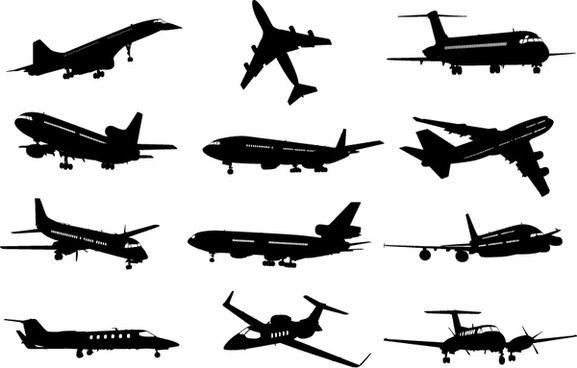
\includegraphics[width=0.9\textwidth]{cover}
\end{center}

\pagebreak

\tableofcontents
 
\pagebreak

\section{Introduction}

Sharks are a part of the chondricthyes family.

\subsection{A subsection}

More text.

\section{Airplanes}

An airplane is defined as a python dictionary. This dictionary should be stored in src>airplanes>"name">plane.py file. The dictionary should have the name plane. There is an example file in the src>airplanes>example directory. The plane dictionary includes many components as key value pairs. There are also nested key value pairs that indicate parent-child relationships. The plane includes a wings, a fuselage, propulsion, weights. The following sections define the ky value pairs and thier contents.

\subsection{Wings}

More text.

\subsubsection{Flaps}

More text.
\begin{center}
    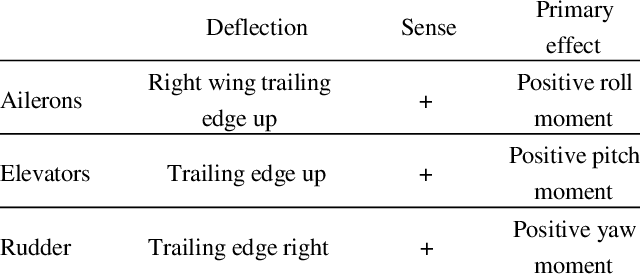
\includegraphics[width=0.6\textwidth]{cs_sign_conventions}
\end{center}

\subsection{Fuselage}

More text.

\section{Analysis}

Your text goes here.

\subsection{Balanced Field Length}

More text.

\subsection{Range}

More text.

\subsection{Specific Excess Power}

More text.

\subsection{Trim}

More text.

\subsubsection{Linear Trims}

More text.

\subsubsection{Non-Linear Trims}

Various nonlinear trim routines are available in this software package. Thses are available through the scipy.optimize.minimize function. 

\section{Modeling}

Your text goes here.

\subsection{Aerodynamics}

There are currently two aerodynamic modeling methods. The first is using DATCOM, and the latter is using the Mark Drela Athena Vortex Lattice software. Note that only lifting surfaces are modeled in AVL, other components like fuselages and langing gear are modeled with DATCOM methods. The long term vision of this package is to provide four aerodynamic modeling methods, DATCOM, panel method, inviscid method (CART3D), and viscous method (SU2, Overflow, or FUN3D).

\subsection{Athena Vortex Lattice}

Link to MIT Athena Vortex Lattice Method (AVL): \\
\url{http://web.mit.edu/drela/Public/web/avl/}

AVL.exe is included in the repository, and should be added to the PATH of your system. The resulting data from AVL is obtained using the avlwrapper API. 

\subsection{Propulsion}

More text.

\subsection{Mass Properties}

More text.

\section{Common}

Your text goes here.

\subsection{Atmosphere}

More text.
\begin{center}
    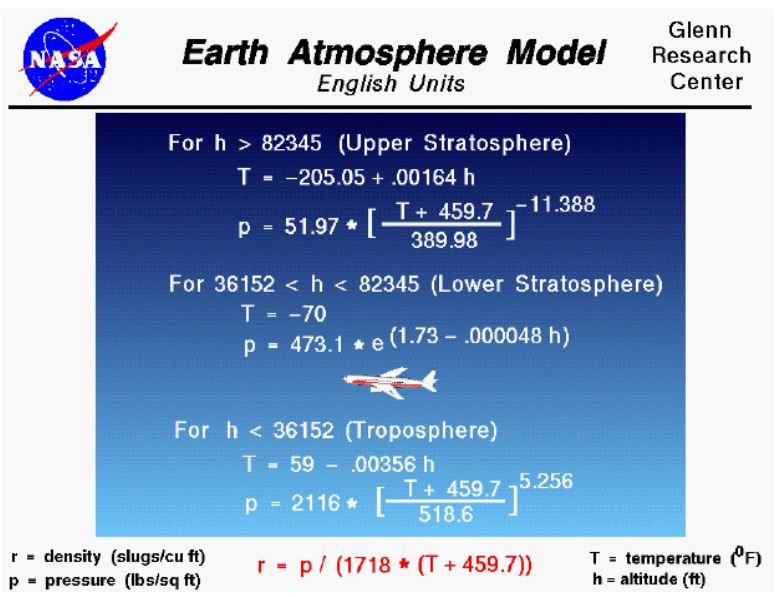
\includegraphics[width=1\textwidth]{atmosphere}
\end{center}

\subsection{Earth}

More text.

\subsection{Equations of Motion}

More text.

\subsection{Rotations}

More text.

\pagebreak

\begin{thebibliography}{9}
\bibitem{latexcompanion} 
Douglas Wells, Bryce Horvath, Linwood McCullers. 
\textit{TM-2017-219627 The Flight Optimization System Weights Estimation Method}. 
NASA, Hampton, VA, 2017.

\bibitem{latexcompanion} 
McDonnell Douglas Corporation. 
\textit{United States Air Force Stability and Control DATCOM}. 
USAF, OH, 1977.
\end{thebibliography}


\end{document}
